\documentclass[aspectratio=169]{beamer}
\usetheme{Madrid}
\usecolortheme{default}

% Packages
\usepackage[utf8]{inputenc}
\usepackage[T1]{fontenc}
\usepackage{graphicx}
\usepackage{amsmath,amsfonts,amssymb}
\usepackage{tikz}
\usetikzlibrary{shapes,arrows,positioning,calc,shadows,decorations.pathmorphing,decorations.markings,patterns}
\usepackage{booktabs}
\usepackage{multirow}
\usepackage{listings}
\usepackage{xcolor}
\usepackage{tcolorbox}
\tcbuselibrary{skins,breakable}

% Code listing style
\lstdefinestyle{python}{
    backgroundcolor=\color{gray!10},
    basicstyle=\ttfamily\footnotesize,
    breaklines=true,
    commentstyle=\color{green!60!black},
    keywordstyle=\color{blue},
    stringstyle=\color{orange!80!black},
    numbers=left,
    numberstyle=\tiny\color{gray},
    numbersep=5pt,
    frame=single,
    framesep=5pt,
    language=Python
}

% Title information
\title[Gamified Doodle Recognition]{Gamified Doodle Recognition for English Vocabulary Acquisition using Deep Learning}
\subtitle{Computer Vision Final Project}
\author[Team]{
    Valent Nathanael (2702343706) \and
    Dimas Putra Aryawan (2702262242) \and
    Yehezkiel Kenneth Hosea (2702352010) \and
    Ivan Feri Budiman (2702377606) \and
    B Orten Subianto Sutanto (2702256372)
}
\institute[BINUS University]{
    BINUS University\\
    School of Computer Science\\
    Computer Science Department
}
\date{\today}

% Custom colors - Vibrant palette
\definecolor{binusblue}{RGB}{0,51,102}
\definecolor{brightblue}{RGB}{41,128,185}
\definecolor{brightgreen}{RGB}{39,174,96}
\definecolor{brightorange}{RGB}{230,126,34}
\definecolor{brightpurple}{RGB}{142,68,173}
\definecolor{brightred}{RGB}{231,76,60}
\definecolor{brightyellow}{RGB}{241,196,15}
\definecolor{lightgray}{RGB}{236,240,241}
\definecolor{darkgray}{RGB}{52,73,94}

\setbeamercolor{structure}{fg=binusblue}
\setbeamercolor{block title}{bg=brightblue,fg=white}
\setbeamercolor{block body}{bg=brightblue!10,fg=black}
\setbeamercolor{block title alerted}{bg=brightorange,fg=white}
\setbeamercolor{block body alerted}{bg=brightorange!10,fg=black}
\setbeamercolor{block title example}{bg=brightgreen,fg=white}
\setbeamercolor{block body example}{bg=brightgreen!10,fg=black}

% Add shadows to blocks
\setbeamertemplate{blocks}[rounded][shadow=true]

\begin{document}

% Title slide
\begin{frame}
    \titlepage
\end{frame}

% Team Members
\begin{frame}{Team Members}
    \centering
    \includegraphics[width=0.95\textwidth,height=0.75\textheight,keepaspectratio]{team_photo.png}
\end{frame}

% Outline
\begin{frame}{Outline}
    \tableofcontents
\end{frame}

% ============================================================================
% SECTION 1: INTRODUCTION
% ============================================================================
\section{Introduction}

\begin{frame}{Background}
    \begin{center}
    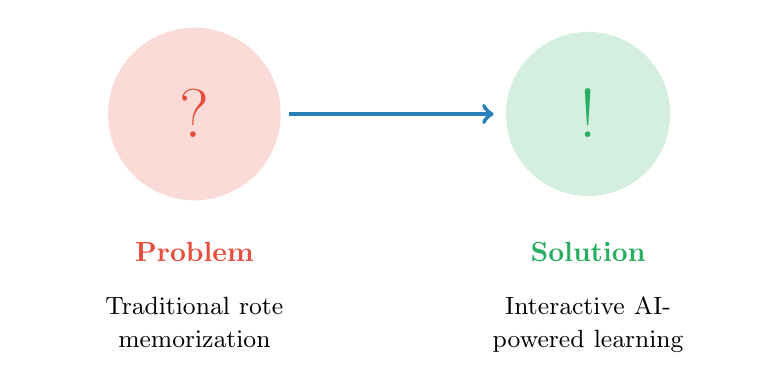
\begin{tikzpicture}
        \node[circle,fill=brightred!20,inner sep=15pt] at (0,0) {\Huge \textcolor{brightred}{?}};
        \node[below] at (0,-1.5) {\textbf{\textcolor{brightred}{Problem}}};
        \node[below,text width=4cm,align=center] at (0,-2.2) {\small Traditional rote memorization};
        
        \node[circle,fill=brightgreen!20,inner sep=15pt] at (5,0) {\Huge \textcolor{brightgreen}{!}};
        \node[below] at (5,-1.5) {\textbf{\textcolor{brightgreen}{Solution}}};
        \node[below,text width=4cm,align=center] at (5,-2.2) {\small Interactive AI-powered learning};
        
        \draw[->,ultra thick,brightblue] (1.2,0) -- (3.8,0);
    \end{tikzpicture}
    \end{center}
    
    \vspace{0.3cm}
    \begin{exampleblock}{\centering \textbf{Our Innovation}}
        \centering
        Real-time doodle recognition with \textcolor{brightgreen}{\textbf{immediate feedback}}, transforming vocabulary into an \textcolor{brightorange}{\textbf{interactive game}}
    \end{exampleblock}
    
    \vspace{0.2cm}
    \begin{center}
        \small \textcolor{darkgray}{Inspired by Google's Quick, Draw! experiment}
    \end{center}
\end{frame}

\begin{frame}{Motivation}
    \begin{columns}
        \column{0.5\textwidth}
        \begin{tcolorbox}[colback=brightred!10,colframe=brightred,title={\textcolor{white}{\textbf{Challenges}}}]
        \small
        \begin{itemize}
            \item Low engagement in traditional methods
            \item Poor retention rates
            \item Lack of immediate feedback
            \item Limited interactivity
        \end{itemize}
        \end{tcolorbox}
        
        \column{0.5\textwidth}
        \begin{tcolorbox}[colback=brightgreen!10,colframe=brightgreen,title={\textcolor{white}{\textbf{Opportunities}}}]
        \small
        \begin{itemize}
            \item AI advances in image recognition
            \item Transfer learning capabilities
            \item Real-time processing
            \item Easy web deployment
        \end{itemize}
        \end{tcolorbox}
    \end{columns}
    
    \vspace{0.3cm}
    \begin{center}
    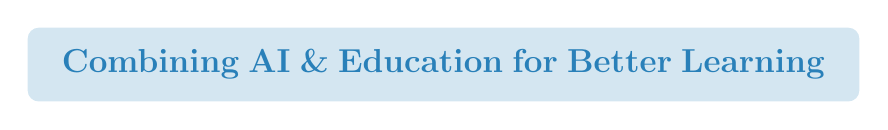
\begin{tikzpicture}
        \node[fill=brightblue!20,rounded corners,inner sep=8pt,text width=10cm,align=center] {
            \large \textcolor{brightblue}{\textbf{Combining AI \& Education for Better Learning}}
        };
    \end{tikzpicture}
    \end{center}
\end{frame}

\begin{frame}{Project Objectives}
    \begin{center}
    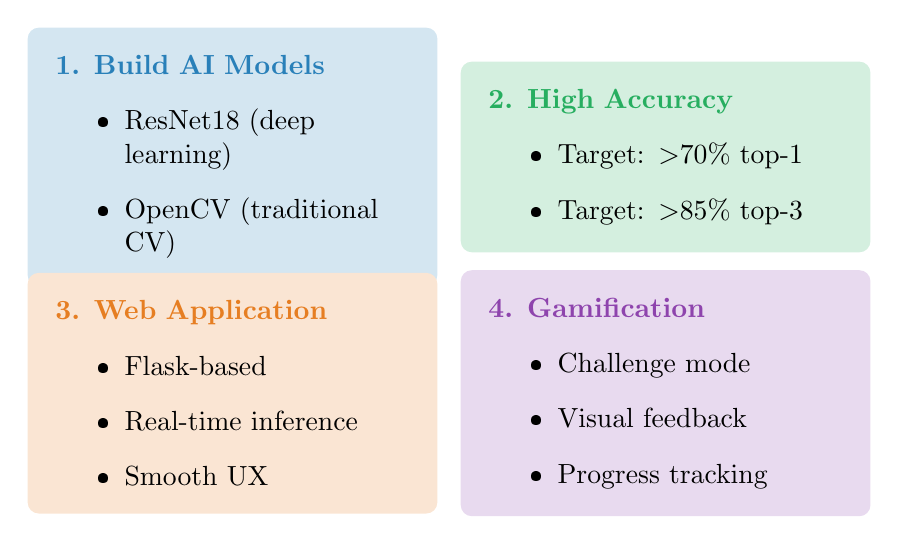
\begin{tikzpicture}
        % Objective 1
        \node[rectangle,fill=brightblue!20,rounded corners,inner sep=10pt,text width=4.5cm] at (0,1.5) {
            \textbf{\textcolor{brightblue}{1. Build AI Models}}
            \begin{itemize}
                \item ResNet18 (deep learning)
                \item OpenCV (traditional CV)
            \end{itemize}
        };
        
        % Objective 2
        \node[rectangle,fill=brightgreen!20,rounded corners,inner sep=10pt,text width=4.5cm] at (5.5,1.5) {
            \textbf{\textcolor{brightgreen}{2. High Accuracy}}
            \begin{itemize}
                \item Target: $>$70\% top-1
                \item Target: $>$85\% top-3
            \end{itemize}
        };
        
        % Objective 3
        \node[rectangle,fill=brightorange!20,rounded corners,inner sep=10pt,text width=4.5cm] at (0,-1.5) {
            \textbf{\textcolor{brightorange}{3. Web Application}}
            \begin{itemize}
                \item Flask-based
                \item Real-time inference
                \item Smooth UX
            \end{itemize}
        };
        
        % Objective 4
        \node[rectangle,fill=brightpurple!20,rounded corners,inner sep=10pt,text width=4.5cm] at (5.5,-1.5) {
            \textbf{\textcolor{brightpurple}{4. Gamification}}
            \begin{itemize}
                \item Challenge mode
                \item Visual feedback
                \item Progress tracking
            \end{itemize}
        };
    \end{tikzpicture}
    \end{center}
\end{frame}

% ============================================================================
% SECTION 2: DATASET
% ============================================================================
\section{Dataset}

\begin{frame}{QuickDraw Dataset}
    \begin{center}
    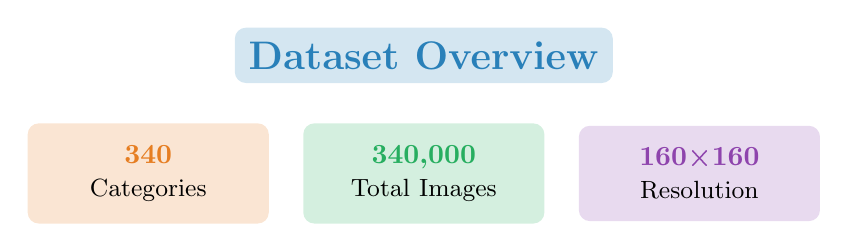
\begin{tikzpicture}
        % Title decoration
        \node[fill=brightblue!20,rounded corners,inner sep=5pt] at (0,2.5) {
            \Large \textcolor{brightblue}{\textbf{Dataset Overview}}
        };
        
        % Main stats boxes
        \node[rectangle,fill=brightorange!20,rounded corners,inner sep=8pt,text width=2.5cm,align=center] at (-3.5,1) {
            \textbf{\textcolor{brightorange}{340}} \\ \small Categories
        };
        \node[rectangle,fill=brightgreen!20,rounded corners,inner sep=8pt,text width=2.5cm,align=center] at (0,1) {
            \textbf{\textcolor{brightgreen}{340,000}} \\ \small Total Images
        };
        \node[rectangle,fill=brightpurple!20,rounded corners,inner sep=8pt,text width=2.5cm,align=center] at (3.5,1) {
            \textbf{\textcolor{brightpurple}{160×160}} \\ \small Resolution
        };
    \end{tikzpicture}
    \end{center}
    
    \vspace{0.3cm}
    \begin{columns}
        \column{0.5\textwidth}
        \begin{exampleblock}{Data Split}
            \centering
            Train: \textbf{70\%} \\
            Validation: \textbf{15\%} \\
            Test: \textbf{15\%}
        \end{exampleblock}
        
        \column{0.5\textwidth}
        \begin{block}{Characteristics}
            \small
            Hand-drawn sketches\\
            High variability\\
            Diverse styles
        \end{block}
    \end{columns}
\end{frame}

\begin{frame}{Sample Categories}
    \centering
    \begin{columns}
        \column{0.25\textwidth}
        \centering
        \includegraphics[width=0.8\textwidth]{../proposal-dl/airplane_sample.png}\\
        \small Airplane
        
        \column{0.25\textwidth}
        \centering
        \includegraphics[width=0.8\textwidth]{../proposal-dl/cat_sample.png}\\
        \small Cat
        
        \column{0.25\textwidth}
        \centering
        \includegraphics[width=0.8\textwidth]{../proposal-dl/app_demo.png}\\
        \small Application
        
        \column{0.25\textwidth}
        \centering
        \textbf{340 Categories}\\
        \vspace{0.3cm}
        \footnotesize
        Animals, Objects,\\
        Food, Vehicles,\\
        Shapes, Actions,\\
        and more...
    \end{columns}
    
    \vspace{0.2cm}
    \begin{block}{Category Examples}
        \tiny
        airplane, apple, banana, basketball, bear, bicycle, bird, book, butterfly, cake, car, cat, chair, clock, cloud, coffee cup, dog, door, eye, face, fish, flower, guitar, hammer, hat, house, key, leaf, moon, mountain, mushroom, pants, pencil, piano, pizza, rainbow, scissors, shoe, smile, snowflake, star, sun, table, telephone, tree, umbrella, violin, wheel, and 292 more...
    \end{block}
\end{frame}

% ============================================================================
% SECTION 3: METHODOLOGY
% ============================================================================
\section{Methodology}

\begin{frame}{Approach Overview}
    \begin{columns}
        \column{0.5\textwidth}
        \textbf{Two Approaches:}
        \begin{enumerate}
            \item \textcolor{blue}{\textbf{Deep Learning}}
            \begin{itemize}
                \item ResNet18 + Transfer Learning
                \item Pre-trained on ImageNet
                \item Fine-tuned for 340 classes
            \end{itemize}
            
            \item \textcolor{orange}{\textbf{Traditional CV}}
            \begin{itemize}
                \item OpenCV Similarity Matching
                \item Template matching
                \item Feature descriptors (SIFT/ORB)
                \item Baseline comparison
            \end{itemize}
        \end{enumerate}
        
        \column{0.5\textwidth}
        \begin{block}{Why Two Approaches?}
            \begin{itemize}
                \item Compare deep learning vs traditional methods
                \item Understand trade-offs
                \item Provide interpretable baseline
                \item Educational value
            \end{itemize}
        \end{block}
    \end{columns}
\end{frame}

\begin{frame}{Data Preprocessing Pipeline}
    \small
    \begin{enumerate}
        \item \textbf{Resize}: 28×28 → 160×160 pixels
        \item \textbf{Grayscale to RGB}: Convert for transfer learning
        \item \textbf{Normalization}: ImageNet statistics
        \begin{itemize}
            \item Mean: [0.485, 0.456, 0.406], Std: [0.229, 0.224, 0.225]
        \end{itemize}
    \end{enumerate}
    
    \vspace{0.3cm}
    \begin{block}{Data Augmentation (Training Only)}
        \small
        \begin{itemize}
            \item Random crop with padding
            \item Random horizontal flip (50\%)
            \item Random rotation (±15°)
            \item Random affine transformations
            \item Color jitter (brightness, contrast)
        \end{itemize}
    \end{block}
    
    \begin{alertblock}{Critical}
        \small
        Proper normalization essential! Wrong values degrade accuracy.
    \end{alertblock}
\end{frame}

\begin{frame}{Model Architecture: ResNet18}
    \small
    \begin{columns}
        \column{0.5\textwidth}
        \begin{block}{Architecture}
            \small
            \begin{itemize}
                \item \textbf{Backbone}: ResNet18 (pre-trained)
                \item \textbf{Input}: 160×160×3 RGB
                \item \textbf{Features}: 512-dim
                \item \textbf{Classifier Head}:
                \begin{itemize}
                    \item Dropout(0.5) + FC(512)
                    \item BatchNorm + ReLU
                    \item Dropout(0.3) + FC(340)
                \end{itemize}
            \end{itemize}
        \end{block}
        
        \column{0.5\textwidth}
        \begin{block}{Training Config}
            \small
            \begin{itemize}
                \item \textbf{Optimizer}: AdamW
                \item \textbf{LR}: 1e-4 (backbone), 1e-3 (head)
                \item \textbf{Batch}: 64, \textbf{Epochs}: 20-30
                \item \textbf{Loss}: CE + Label Smoothing
                \item \textbf{Scheduler}: Cosine Annealing
            \end{itemize}
        \end{block}
        
        \vspace{0.2cm}
        \begin{block}{Transfer Learning}
            \small
            \begin{itemize}
                \item Freeze backbone initially
                \item Train classifier, then fine-tune all
            \end{itemize}
        \end{block}
    \end{columns}
\end{frame}

\begin{frame}{ResNet18 Architecture Diagram}
    \centering
    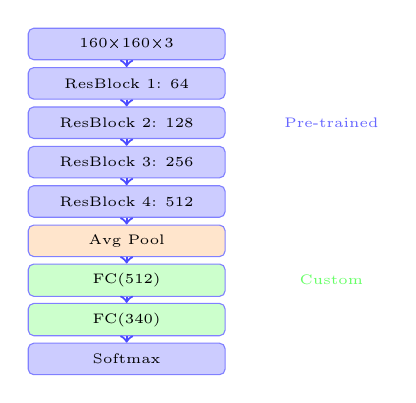
\begin{tikzpicture}[
        node distance=0.5cm,
        block/.style={rectangle, draw=blue!50, fill=blue!20, minimum width=2.5cm, minimum height=0.4cm, text centered, font=\tiny, rounded corners=2pt},
        arrow/.style={->, thick, color=blue!70}
    ]
    
    \node[block] (input) {160×160×3};
    \node[block, below of=input] (res1) {ResBlock 1: 64};
    \node[block, below of=res1] (res2) {ResBlock 2: 128};
    \node[block, below of=res2] (res3) {ResBlock 3: 256};
    \node[block, below of=res3] (res4) {ResBlock 4: 512};
    \node[block, below of=res4, fill=orange!20] (gap) {Avg Pool};
    \node[block, below of=gap, fill=green!20] (fc1) {FC(512)};
    \node[block, below of=fc1, fill=green!20] (fc2) {FC(340)};
    \node[block, below of=fc2] (output) {Softmax};
    
    \draw[arrow] (input) -- (res1);
    \draw[arrow] (res1) -- (res2);
    \draw[arrow] (res2) -- (res3);
    \draw[arrow] (res3) -- (res4);
    \draw[arrow] (res4) -- (gap);
    \draw[arrow] (gap) -- (fc1);
    \draw[arrow] (fc1) -- (fc2);
    \draw[arrow] (fc2) -- (output);
    
    \node[right of=res2, node distance=2.6cm, text=blue!60, font=\tiny] {Pre-trained};
    \node[right of=fc1, node distance=2.6cm, text=green!60, font=\tiny] {Custom};
    
    \end{tikzpicture}
    
    \begin{block}{\footnotesize 11.6M params (438K trainable)}
    \end{block}
\end{frame}

\begin{frame}{OpenCV Similarity Matching}
    \small
    \begin{columns}
        \column{0.5\textwidth}
        \textbf{Methods:}
        \begin{enumerate}
            \item \textbf{Template Matching}
            \begin{itemize}
                \item Normalized cross-correlation
            \end{itemize}
            
            \item \textbf{Feature Matching}
            \begin{itemize}
                \item SIFT/ORB keypoints
            \end{itemize}
            
            \item \textbf{Histogram Comparison}
            \begin{itemize}
                \item Statistical distribution
            \end{itemize}
        \end{enumerate}
        
        \column{0.5\textwidth}
        \begin{block}{Preprocessing}
            \small
            \textbf{Sobel Edge Detection}
            \begin{itemize}
                \item Extract edges
                \item Reduce noise
                \item Improve matching
            \end{itemize}
        \end{block}
        
        \begin{block}{Multi-Method Fusion}
            \small
            \begin{itemize}
                \item Combine all methods
                \item Weighted voting
            \end{itemize}
        \end{block}
    \end{columns}
    
    \vspace{0.2cm}
    \begin{alertblock}{Limitation}
        \small
        Traditional CV struggles with sketch variability. Accuracy: ~16\% vs 75\% for ResNet.
    \end{alertblock}
\end{frame}

% ============================================================================
% SECTION 4: RESULTS
% ============================================================================
\section{Results}

\begin{frame}{Model Performance Comparison}
    \begin{table}[h]
    \centering
    \begin{tabular}{lcc}
    \toprule
    \textbf{Model} & \textbf{Top-1 Accuracy} & \textbf{Top-3 Accuracy} \\
    \midrule
    \textbf{ResNet18} & \textcolor{green}{\textbf{75.03\%}} & \textcolor{green}{\textbf{90.70\%}} \\
    OpenCV Similarity & 16.2\% & -- \\
    \midrule
    \textbf{Target} & $>$70\% & $>$85\% \\
    \bottomrule
    \end{tabular}
    \end{table}
    
    \vspace{0.3cm}
    \begin{columns}
        \column{0.5\textwidth}
        \begin{exampleblock}{Achievements}
            \small
            \begin{itemize}
                \item Top-1: \textbf{75\%} (target: 70\%)
                \item Top-3: \textbf{90.7\%} (target: 85\%)
                \item Inference: \textbf{~400ms}
                \item Model: \textbf{~45MB}
            \end{itemize}
        \end{exampleblock}
        
        \column{0.5\textwidth}
        \begin{block}{Training Info}
            \small
            \begin{itemize}
                \item 340,000 images
                \item 340 categories
                \item 70/15/15\% split
                \item ~4-6 hours (GPU)
            \end{itemize}
        \end{block}
    \end{columns}
\end{frame}

\begin{frame}{Per-Class Performance Analysis}
    \begin{columns}
        \column{0.5\textwidth}
        \begin{tcolorbox}[colback=brightgreen!10,colframe=brightgreen,title={\textcolor{white}{\textbf{Top Performers}}}]
        \small
        \begin{itemize}
            \item Angel: \textbf{97\%}
            \item Mona Lisa: \textbf{90\%}
            \item Eiffel Tower: \textbf{90\%}
            \item Many $>$85\%
        \end{itemize}
        \end{tcolorbox}
        
        \vspace{0.2cm}
        \begin{tcolorbox}[colback=brightorange!10,colframe=brightorange,title={\textcolor{white}{\textbf{Challenging}}}]
        \small
        \begin{itemize}
            \item Great Wall: 49\%
            \item Asparagus: 43\%
            \item Abstract concepts
        \end{itemize}
        \end{tcolorbox}
        
        \column{0.5\textwidth}
        \begin{center}
        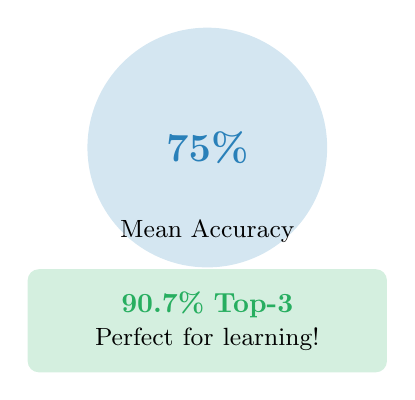
\begin{tikzpicture}
            \node[circle,fill=brightblue!20,inner sep=20pt] at (0,1) {
                \Large \textbf{\textcolor{brightblue}{75\%}}
            };
            \node[below] at (0,0.2) {\small Mean Accuracy};
            
            \node[rectangle,fill=brightgreen!20,rounded corners,inner sep=8pt,text width=4cm,align=center] at (0,-1.2) {
                \textbf{\textcolor{brightgreen}{90.7\% Top-3}}\\
                \small Perfect for learning!
            };
        \end{tikzpicture}
        \end{center}
    \end{columns}
\end{frame}

\begin{frame}{Confusion Matrix Insights}
    \begin{columns}
        \column{0.5\textwidth}
        \begin{block}{Overall Pattern}
            \begin{itemize}
                \item Strong diagonal (correct predictions)
                \item Some confusion between:
                \begin{itemize}
                    \item Similar objects (cat/tiger)
                    \item Abstract concepts
                    \item Objects with similar shapes
                \end{itemize}
            \end{itemize}
        \end{block}
        
        \column{0.5\textwidth}
        \begin{block}{Model Strengths}
            \begin{itemize}
                \item Distinguishes distinct objects well
                \item Handles style variations
                \item Robust to incomplete drawings
                \item Fast inference time
            \end{itemize}
        \end{block}
    \end{columns}
    
    \vspace{0.5cm}
    \centering
    \textcolor{binusblue}{\textbf{The model successfully generalizes across diverse drawing styles and cultural variations}}
\end{frame}

% ============================================================================
% SECTION 5: WEB APPLICATION
% ============================================================================
\section{Web Application}

\begin{frame}{Application Features}
    \begin{center}
    \begin{tikzpicture}
        % Mode 1
        \node[rectangle,fill=brightblue!20,rounded corners,inner sep=12pt,text width=5cm] at (-3,1.5) {
            \textbf{\textcolor{brightblue}{Free-Draw Mode}}
            \begin{itemize}
                \item Real-time recognition
                \item Top-10 suggestions
                \item Practice freely
            \end{itemize}
        };
        
        % Mode 2
        \node[rectangle,fill=brightgreen!20,rounded corners,inner sep=12pt,text width=5cm] at (3,1.5) {
            \textbf{\textcolor{brightgreen}{Challenge Mode}}
            \begin{itemize}
                \item Target word given
                \item Scoring system
                \item Progress tracking
            \end{itemize}
        };
        
        % Tech stack
        \node[rectangle,fill=brightorange!15,rounded corners,inner sep=10pt,text width=10.5cm] at (0,-1.2) {
            \small
            \textbf{⚙️ Tech:} Flask + HTML5 Canvas + PyTorch | 
            \textbf{Speed:} $<$500ms response time
        };
    \end{tikzpicture}
    \end{center}
\end{frame}

\begin{frame}{Application Screenshot}
    \begin{center}
    \begin{tikzpicture}
        \node[inner sep=0] (img) at (0,0.5) {
            \includegraphics[width=0.7\textwidth,height=0.55\textheight,keepaspectratio]{../proposal-dl/app_demo.png}
        };
        
        \node[fill=brightblue!20,rounded corners,inner sep=8pt,text width=11cm,align=center] at (0,-2.8) {
            \textbf{Drawing Canvas} + \textbf{Real-time AI Predictions} + \textbf{Confidence Scores}
        };
    \end{tikzpicture}
    \end{center}
\end{frame}

\begin{frame}{Gamification Elements}
    \begin{center}
    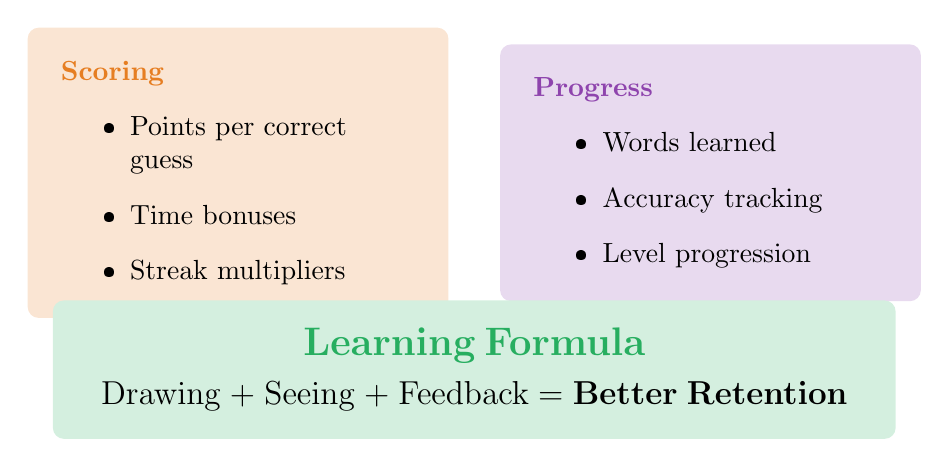
\begin{tikzpicture}
        % Game elements
        \node[rectangle,fill=brightorange!20,rounded corners,inner sep=12pt,text width=4.5cm] at (-3,1) {
            \textbf{\textcolor{brightorange}{Scoring}}
            \begin{itemize}
                \item Points per correct guess
                \item Time bonuses
                \item Streak multipliers
            \end{itemize}
        };
        
        \node[rectangle,fill=brightpurple!20,rounded corners,inner sep=12pt,text width=4.5cm] at (3,1) {
            \textbf{\textcolor{brightpurple}{Progress}}
            \begin{itemize}
                \item Words learned
                \item Accuracy tracking
                \item Level progression
            \end{itemize}
        };
        
        % Learning benefit
        \node[rectangle,fill=brightgreen!20,rounded corners,inner sep=10pt,text width=10cm,align=center] at (0,-1.5) {
            \Large \textcolor{brightgreen}{\textbf{Learning Formula}}\\
            \vspace{0.2cm}
            \large Drawing + Seeing + Feedback = \textbf{Better Retention}
        };
    \end{tikzpicture}
    \end{center}
\end{frame}

% ============================================================================
% SECTION 6: CONCLUSION
% ============================================================================
\section{Conclusion}

\begin{frame}{Key Achievements}
    \begin{center}
    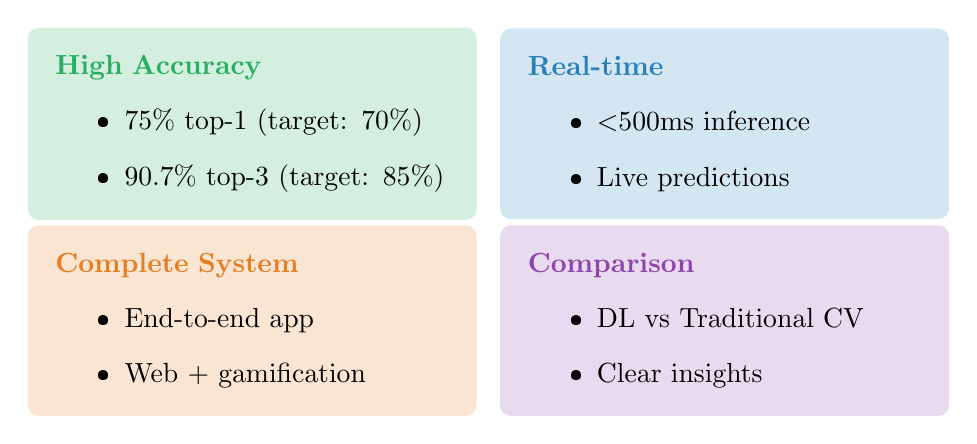
\begin{tikzpicture}
        % Achievement 1
        \node[rectangle,fill=brightgreen!20,rounded corners,inner sep=10pt,text width=5cm] at (-3,2) {
            \textbf{\textcolor{brightgreen}{High Accuracy}}
            \begin{itemize}
                \item 75\% top-1 (target: 70\%)
                \item 90.7\% top-3 (target: 85\%)
            \end{itemize}
        };
        
        % Achievement 2
        \node[rectangle,fill=brightblue!20,rounded corners,inner sep=10pt,text width=5cm] at (3,2) {
            \textbf{\textcolor{brightblue}{Real-time}}
            \begin{itemize}
                \item $<$500ms inference
                \item Live predictions
            \end{itemize}
        };
        
        % Achievement 3
        \node[rectangle,fill=brightorange!20,rounded corners,inner sep=10pt,text width=5cm] at (-3,-0.5) {
            \textbf{\textcolor{brightorange}{Complete System}}
            \begin{itemize}
                \item End-to-end app
                \item Web + gamification
            \end{itemize}
        };
        
        % Achievement 4
        \node[rectangle,fill=brightpurple!20,rounded corners,inner sep=10pt,text width=5cm] at (3,-0.5) {
            \textbf{\textcolor{brightpurple}{Comparison}}
            \begin{itemize}
                \item DL vs Traditional CV
                \item Clear insights
            \end{itemize}
        };
    \end{tikzpicture}
    \end{center}
\end{frame}

\begin{frame}{Technical Contributions}
    \small
    \begin{columns}
        \column{0.5\textwidth}
        \textbf{Model Development:}
        \begin{itemize}
            \item ResNet18 transfer learning
            \item Custom classifier architecture
            \item Optimized training pipeline
        \end{itemize}
        
        \vspace{0.2cm}
        \textbf{System Architecture:}
        \begin{itemize}
            \item Flask backend
            \item Real-time inference
            \item Scalable design
        \end{itemize}
        
        \column{0.5\textwidth}
        \begin{block}{Lessons Learned}
            \small
            \begin{itemize}
                \item \textcolor{red}{\textbf{Critical}}: ImageNet normalization essential
                \item Data augmentation improves generalization
                \item Transfer learning works on sketches
                \item Traditional CV limited here
            \end{itemize}
        \end{block}
        
        \vspace{0.2cm}
        \begin{block}{Best Practices}
            \small
            \begin{itemize}
                \item Proper preprocessing
                \item Stratified splits
                \item Comprehensive metrics
            \end{itemize}
        \end{block}
    \end{columns}
\end{frame}

\begin{frame}{Future Work}
    \small
    \begin{columns}
        \column{0.5\textwidth}
        \textbf{Model Improvements:}
        \begin{itemize}
            \item Stroke-based RNNs
            \item Transformer architectures
            \item Ensemble methods
        \end{itemize}
        
        \vspace{0.2cm}
        \textbf{Application Features:}
        \begin{itemize}
            \item Multiplayer mode
            \item Social sharing
            \item Mobile app version
        \end{itemize}
        
        \column{0.5\textwidth}
        \begin{block}{Research Directions}
            \small
            \begin{itemize}
                \item Cross-cultural drawing analysis
                \item Adaptive difficulty
                \item Personalized learning paths
                \item Curriculum integration
            \end{itemize}
        \end{block}
        
        \vspace{0.2cm}
        \begin{alertblock}{Impact}
            \footnotesize
            Scalable to other languages and domains
        \end{alertblock}
    \end{columns}
\end{frame}

\begin{frame}{Summary}
    \begin{center}
    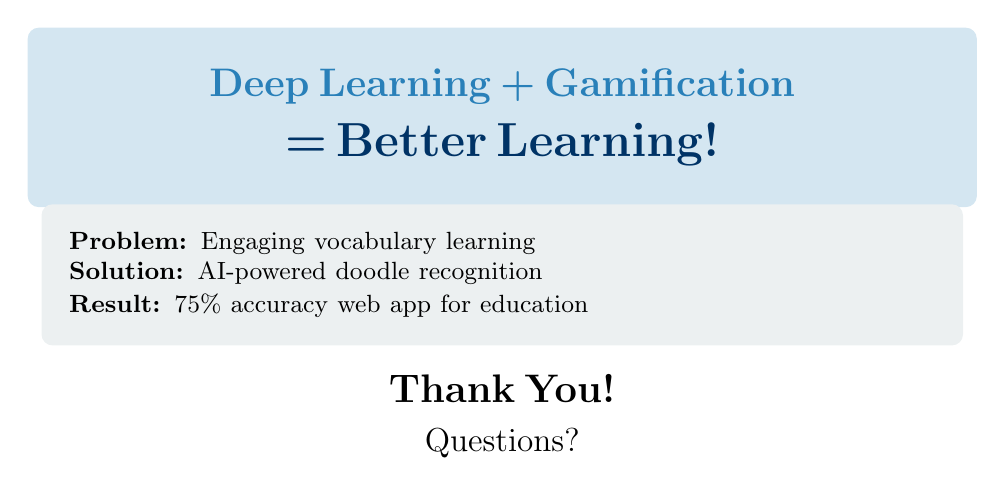
\begin{tikzpicture}
        % Main message
        \node[rectangle,fill=brightblue!20,rounded corners,inner sep=15pt,text width=11cm,align=center] at (0,2) {
            \Large \textcolor{brightblue}{\textbf{Deep Learning + Gamification}}\\
            \vspace{0.2cm}
            \LARGE \textcolor{binusblue}{\textbf{= Better Learning!}}
        };
        
        % Key points
        \node[rectangle,fill=lightgray,rounded corners,inner sep=10pt,text width=11cm] at (0,0) {
            \small
            \textbf{Problem:} Engaging vocabulary learning\\
            \textbf{Solution:} AI-powered doodle recognition\\
            \textbf{Result:} 75\% accuracy web app for education
        };
        
        % Thank you
        \node[text width=11cm,align=center] at (0,-1.8) {
            \Large \textbf{Thank You!}\\
            \vspace{0.2cm}
            \large Questions?
        };
    \end{tikzpicture}
    \end{center}
\end{frame}

\end{document}
